\chapter{狭义相对论中的向量分析}
\label{chap2}

\section{向量的定义}
\label{sec2.1}

\section{向量代数}
\label{sec2.2}

\section{四维速度}
\label{sec2.3}
世界线的四维速度(four-velocity, 简称四速)是一种十分重要的向量。伽利略的三维几何中,速度是与粒子运动轨迹相切的向量。四维几何的四维速度$\vec{U}$定义为与粒子世界线相切的、在粒子的参考系中长度为单位时间的向量。先考虑最简单的匀速直线运动粒子,在与粒子相对静止的惯性系中,根据定义,四维速度向量的方向与时间轴平行、长度为单位时间,这意味着四维速度就等于该系的基向量$\vec{e}_0$。于是,匀速直线运动粒子的四维速度定义为该粒子静止惯性系的基向量$\vec{e}_0$. “四维速度”名字的来历是$\vec{U}$的空间分量与通常所说的粒子的三维速度$\bm{p}$关系密切,参见下面的例子与\eqref{equ2.21}式。


\textit{变速运动的粒子}不存在始终在其中静止的惯性系。然而,\textit{仍然存在着}与粒子瞬时静止的惯性系——它的速度在一瞬间与粒子速度相同(共动参考系),不过在下一时刻就不再是共动的了。这个参考系称为\textit{瞬时共动参考系 (momentarily comoving reference frame,} \textbf{\ MCRF} \textit{)},这个概念极其重要。(实际上,一个粒子在某一特定事件点有无数个MCRF;它们的速度相同,而空间坐标轴相差旋转变换。不过这通常不重要,取哪个空间轴取向的MCRF都行)变速运动粒子(在某一事件点)的四速\textit{定义为}在该事件点的MCRF的基向量$\vec{e}_0$. 该向量与(弯曲的)粒子世界线相切。图\ref{fig2.2}中,粒子在事件$\mathscr{A}$的MCRF是$\MObar$系,图中画出了基向量,$\vec{e}_{\bar{0}}$就是粒子在$\mathscr{A}$点的四速$\vec{U}$.

{
    \centering
    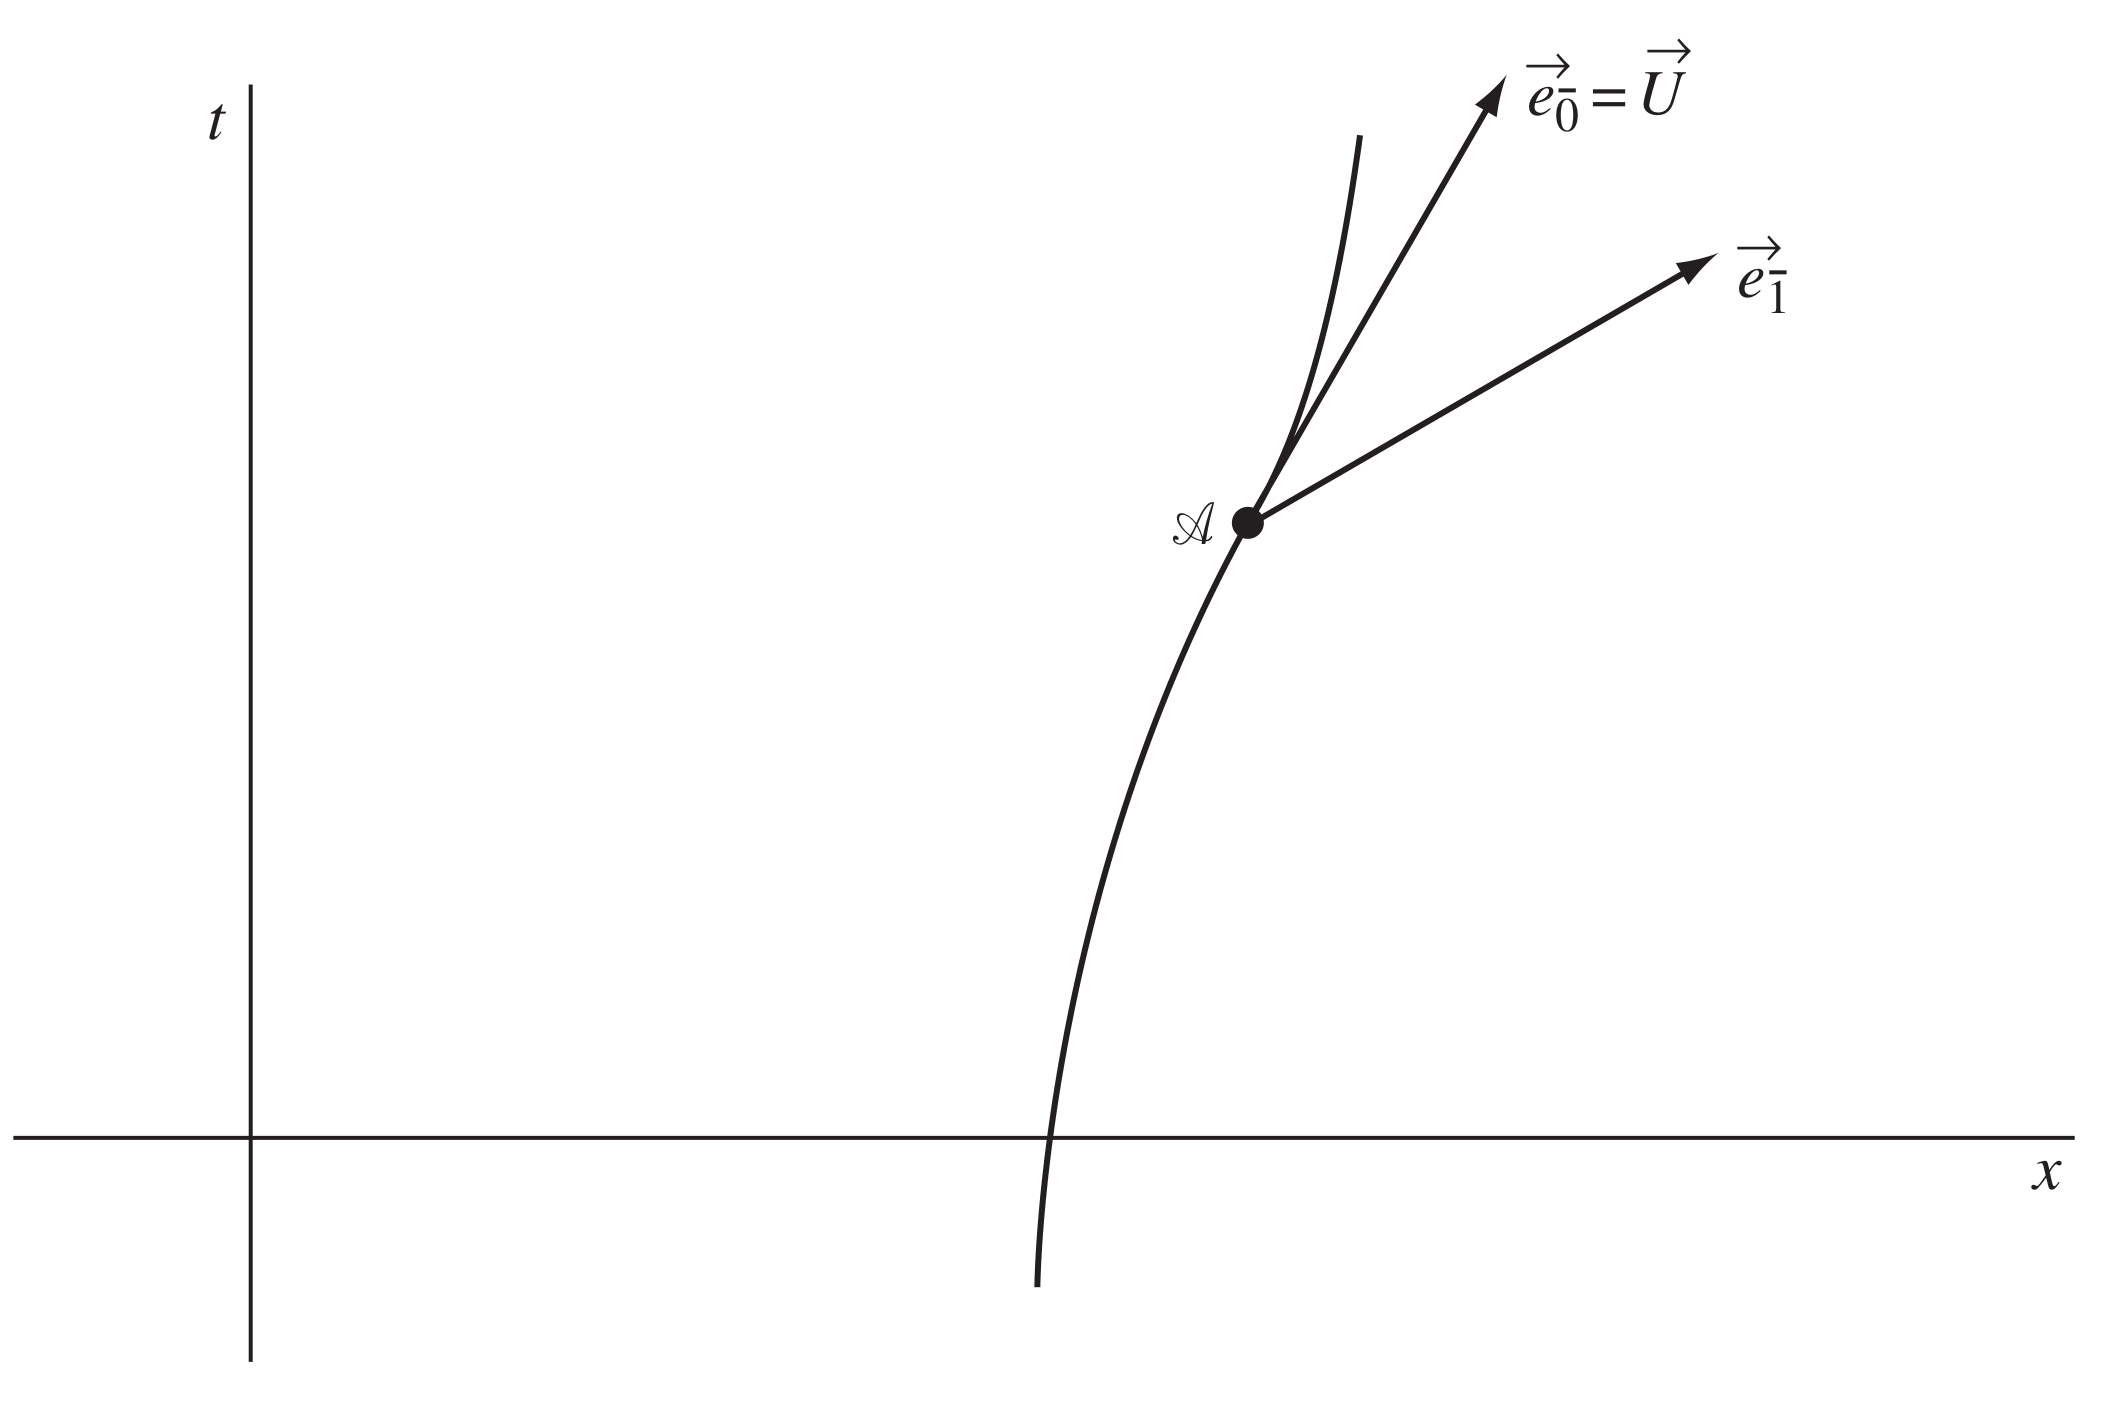
\includegraphics[width=0.7\textwidth]{fig2.2.png}
    \figcaption{\textit{粒子世界线在$\mathscr{A}$点的四维速度与MCRF基向量}}
    \label{fig2.2}
}


\section{四维动量}
\label{sec2.4}
四维动量$\vec{p}$定义为
\begin{shaded}
\begin{equation}
    \vec{p} = m \vec{U},
\label{equ2.19}
\end{equation}
\end{shaded}
其中$m$是粒子的\textit{静止质量 (rest mass,简称静质量)},也就是在粒子静止的坐标系中测得的粒子质量。四动量在任一惯性系$\MO$中的分量记作
\begin{equation}
    \vec{p} \xrightarrow[\MO]{ } (E, p^1, p^2, p^3).
\label{equ2.20}
\end{equation}
分量$p^0$记作$E$,称为粒子在坐标系$\MO$中的\textit{能量 (energy)}。其余分量称为四动量的空间分量$p^i$.

\subsection*{例子}
静质量为$m$的粒子在坐标系$\MO$中沿$x$轴方向运动,速度为$\bm{v}$,粒子四速、四动量在$\MO$系的分量是什么?粒子在其中静止的坐标系记作$\MObar$,该系的时间基向量为$\vec{e}_{\bar{0}}$。根据四速与四动量的定义有
\begin{equation}
\begin{split}
    \vec{U} &= \vec{e}_{\bar{0}}, & \quad \vec{p} &= m\vec{U}, \\
    U^\alpha &= \Lambda\indices{^\alpha_{\bar{\beta}}} ( \vec{e}_{\bar{0}} )^{\bar{\beta}} = \Lambda\indices{^\alpha_{\bar{0}}}, \quad & p^\alpha &= m \Lambda\indices{^\alpha_{\bar{0}}}.
\end{split}
\label{equ2.21}
\end{equation}
由此可得
\begin{align*}
    U^0 &= (1 - v^2)^{-1/2}, \quad & p^0 &= m(1 - v^2)^{-1/2}, \\
    U^1 &= v (1 - v^2)^{-1/2}, \quad & p^1 &= mv (1 - v^2)^{-1/2}, \\
    U^2 &= 0, \quad & p^2 &= 0, \\
    U^3 &= 0, \quad & p^3 &= 0.
\end{align*}
对于很小的$v$,$\vec{U}$的空间分量近似为$(v, 0, 0)$,$\vec{p}$的空间分量为$(mv, 0, 0)$,从这就能看出它们的名字——四维速度、四维动量——的合理性。还是对于很小的$v$,能量近似为:
\begin{equation*}
    E := p^0 = m (1 - v^2)^{-1/2} \approx m + \frac{1}{2} m v^2.
\end{equation*}
它等于静质能(rest-mass energy)与(伽利略形式的)动能之和。

\subsection*{四维动量守恒}
伽利略力学中,粒子的碰撞过程遵从能量、动量守恒定律。因为$\vec{p}$的分量在非相对论极限下退化为伽利略形式的能量、动量,因此很自然地假设在相对论情形下,四维向量$\vec{p}$也守恒。也就是说,几个粒子发生相互作用,粒子的总动量:
\begin{equation}
    \vec{p} := \sum_{\text{所有粒子,编号为}(i)} \vec{p}_{(i)},
\label{equ2.22}
\end{equation}
在碰撞过程的前后不变。($\vec{p}_{(i)}$是第$i$个粒子的动量)

四维动量守恒定律实际上是个额外\textit{假设},因为我们只知道它的非相对论极限是正确的。不过就像SR的两条基本假设那样,四动量守恒经历了丰富的实验验证。至少它预言了能量守恒定律必须包括静质能:静质量可以消灭、相应的能量可以转化为动能从而化为热能。这个预言每天都在被核电站所验证。

上面四动量守恒的陈述中掩藏了很重要的一点:一次碰撞“之前”与“之后”的含义是什么?假设不同的粒子发生了两次碰撞,这两个事件的间隔是类空的,如下图。要将同一时刻的四动量相加,应该沿着等$t$时刻还是等$\bar{t}$时刻?如图\ref{fig2.3}所示,$\MO$系的测量结果为:事件$\mathscr{A}$发生在$t = 0$之前,事件$\mathscr{B}$在之后,因此$t = 0$时刻的总动量等于$\mathscr{A}$之后加上$\mathscr{B}$之前的动量。而在$\MObar$系中,事件$\mathscr{A}, \mathscr{B}$同时发生于时刻$\bar{t} = 0$之前,因此$\bar{t} = 0$时刻的总动量等于事件$\mathscr{A}, \mathscr{B}$之后的动量之和。 甚至还可以找到一个坐标系,在其中事件$\mathscr{B}$比$\mathscr{A}$发生的\textit{更早},and the adding-up may be the reverse of $\MO$'s. 

{
    \centering
    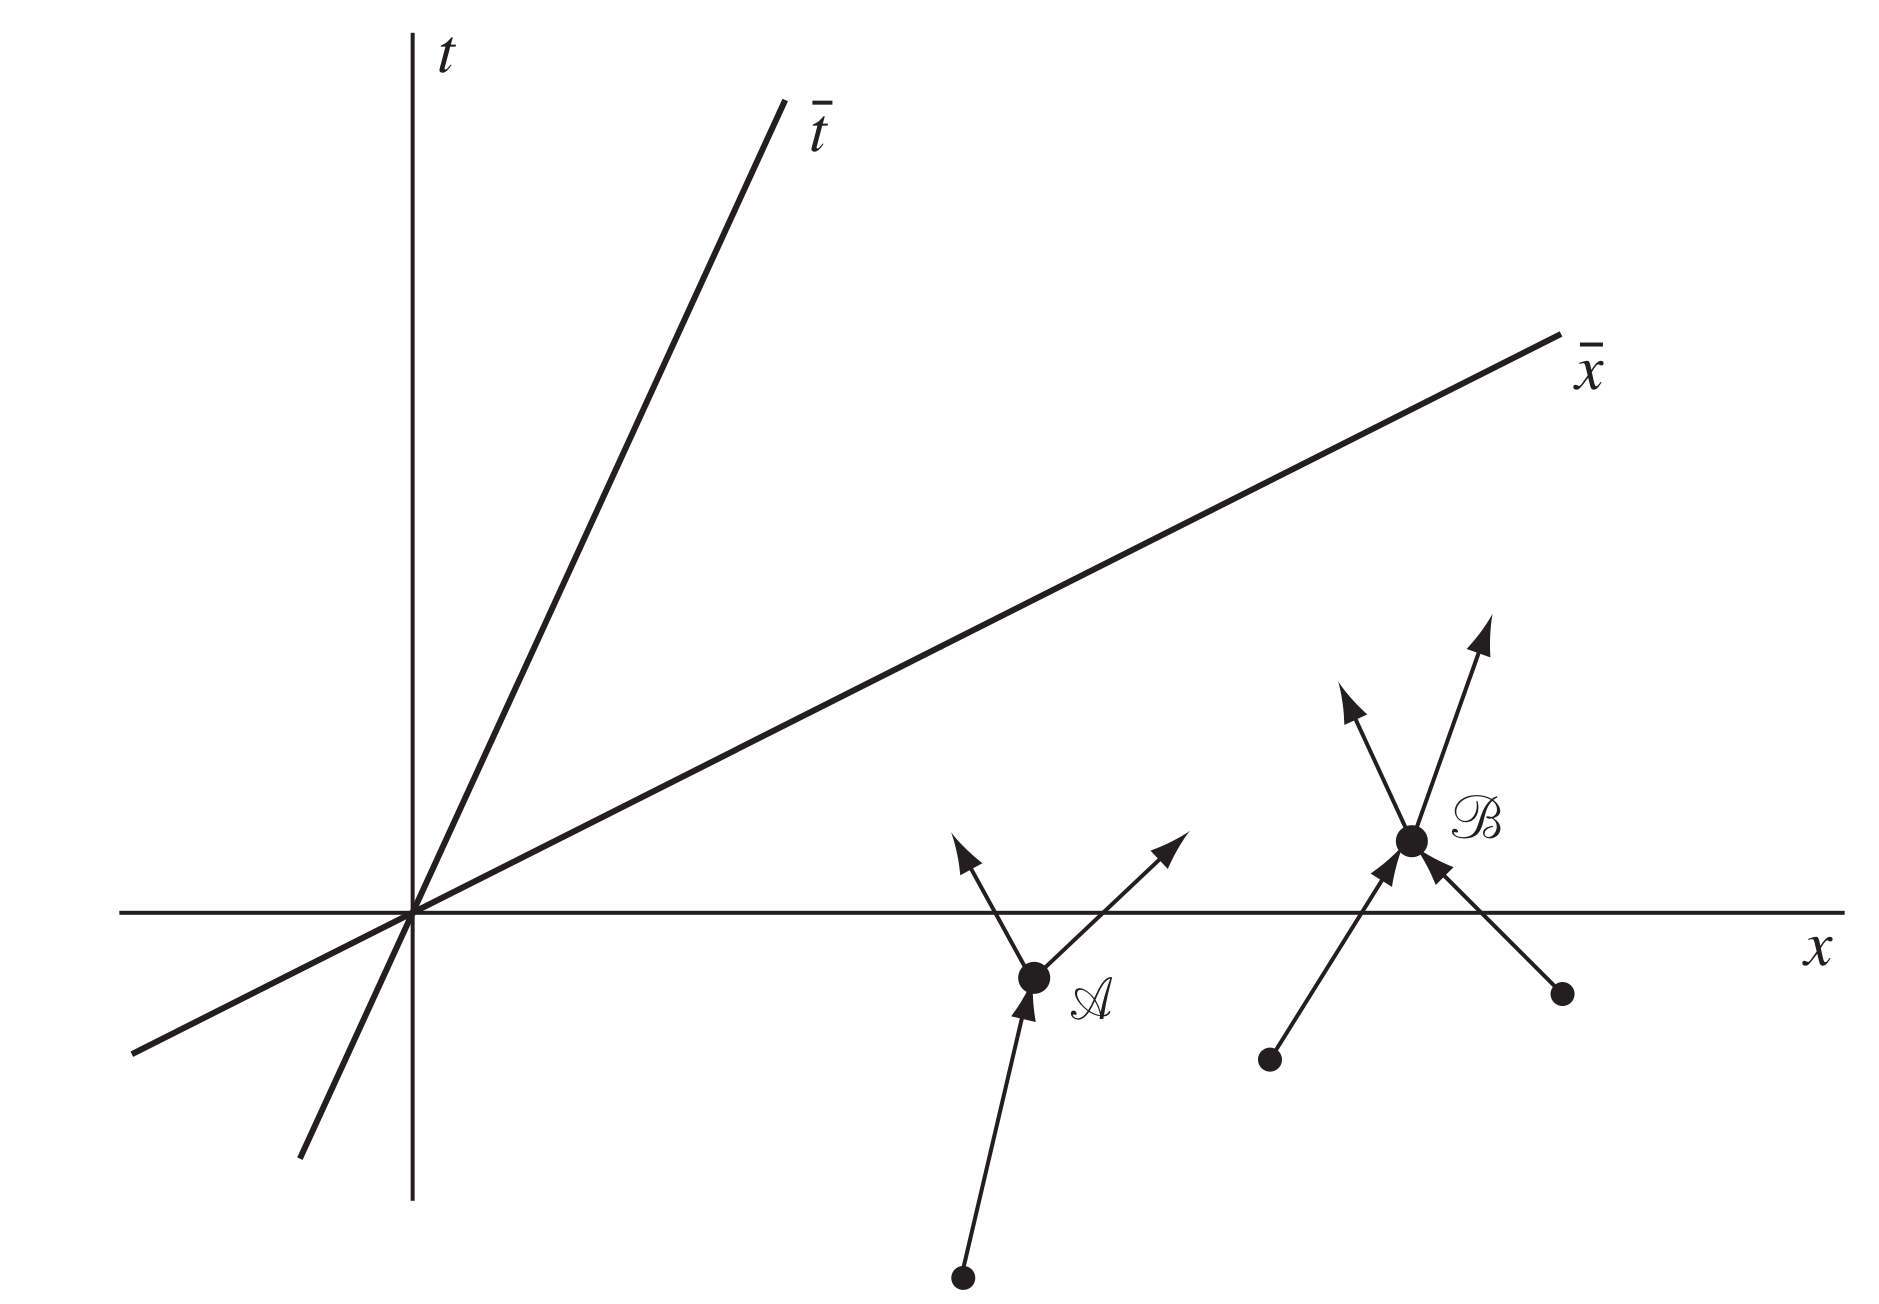
\includegraphics[width=0.7\textwidth]{fig2.3.png}
    \figcaption{\textit{当考虑几个碰撞过程时,组成某一时刻的总动量的各个四动量取决于坐标系,但总的四维动量是在所有坐标系中相同的四维向量;它的分量在坐标系之间的变换规律服从Lorentz变换。}}
    \label{fig2.3}
}

这实际上没问题。既然每个碰撞过程都服从动量守恒,那么事件$\mathscr{A}$之后与之前的动量和相等,事件$\mathscr{B}$也一样。因此\textit{每个}惯性观者都得到相同的总的四动量$\vec{p}$。(它的分量随坐标系的不同而不同,但是它是同一个向量。) 有一点很重要:\textit{任意}观者可以定义他自己的等时线(这实际上是等时的三维空间,称之为四维时空中等时的\textit{超平面}),把那个时刻的所有动量相加,得到的向量与其他任何观者的结果都相同。理解这一点十分重要,因为这种守恒律会在之后再次出现。

\subsection*{质心 (CM) 系}
质心系(center of momentum frame, CM)是总动量的空间分量在其中为零的惯性系:
\begin{equation}
    \sum_i \vec{p}_{(i)} \xrightarrow[\text{CM}]{ } (E_{\text{TOTAL}}, 0, 0, 0).
\label{equ2.23}
\end{equation}
与MCRF同理,任意相对于CM系静止的坐标系也是CM系。

\section{标量积}
\label{sec2.5}

\section{应用}
\label{sec2.6}

\section{光子}
\label{sec2.7}

\section{扩展阅读}
\label{sec2.8}

\section{习题}
\label{sec2.9}